%% *************************************************************************
%%
%% This is a derivative work of the RIT Space Exploration Standard defining
%% guidelines for content and formatting of project design documents.
%%
%% This document uses IEEEtran.cls, the official IEEE LaTeX class
%% for authors of the Institute of Electrical and Electronics Engineers
%% (IEEE) Transactions journals and conferences.
%%
%% *************************************************************************

%% *************************************************************************
% LaTeX REFERENCES
% ----------------
%   Intro to LaTeX: http://www.rpi.edu/dept/arc/docs/latex/latex-intro.pdf
%   Comprehensive LaTeX symbol list: http://tug.ctan.org/info/symbols/comprehensive/symbols-a4.pdf
%% *************************************************************************

% tell \LaTeX what kind of formatting to use
\documentclass[conference]{IEEEtran} % http://www.ctan.org/pkg/ieeetran
\usepackage{blindtext} % enable placeholder text generator
\usepackage{graphicx} % enable toolbox for embedding figures and pictures
\usepackage{nomencl} % enable package for adding a list of variables and constants at the beginning, aka "nomenclature"
\usepackage{siunitx} % enable package for easily formatting units
\usepackage{hyperref} % enable package for cross-referencing figures, sections, references etc.
% how to use hyperref: http://www2.washjeff.edu/users/rhigginbottom/latex/resources/lecture09.pdf
\usepackage[T1]{fontenc} % change text encoding to make it more crisp
\usepackage{etoolbox} % enable conditionals for help text
\usepackage{booktabs} % make beautiful tables!

% initialize nomenclature package
\makenomenclature{}

% set title. choose something as descriptive and precise as possible. Descriptive > sounding cool. remember this!
\title{Foundation for Development of RIT SPEX Astro Tracking Team}


\author{
  % List the authors of the design document. The Champion should go first.
  % The \$~\$ markers tell \LaTeX{} to treat the text inside to be treated as a math expression. This way you can use operators like \textcaret{} to place characters as superscripts.
  % Some \LaTeX{} templates handle the author block in different ways. For example, the \href{http://www.worldscientific.com/worldscinet/jai}{Journal of Astronomical Instrumentation} requires the authors' addresses and emails to be included as well.
  % The \textbackslash{}thanks command puts the contents inside those brackets in a footnote at the bottom of the first page. Technically speaking, \textbackslash{}thanks is just a specially formatted footnote.
  % IEEE also has a ``long form'' author block for many authors. Check here for more information:
  % \url{https://tex.stackexchange.com/questions/156523/multiple-authors-with-common-affiliations-in-ieeetran-conference-template}
  % Read here for a more advanced options to modifying footnotes in the author block:  \url{http://tex.stackexchange.com/questions/826/symbols-instead-of-numbers-as-footnote-markers}
  %   Here, we use the IEEE long-form author block.
  \IEEEauthorblockN{% This block is for author Names.
    Evan~Putnam\IEEEauthorrefmark{1},  %the number in the bracket is a reference number to identify this footnote. \LaTeX will figure out what symbol to put there.
    Marilyn~Wolbert\IEEEauthorrefmark{2}
  }
  \IEEEauthorblockA{% This block is for the author Affiliations, aka department and university
    RIT Space Exploration, Rochester Institute of Technology \\ %\\ starts a new line
    Rochester, N.Y. \\
    Email:
    \IEEEauthorrefmark{1}emp9173@rit.edu,
    \IEEEauthorrefmark{2}mxw3196@rit.edu
  }
  %%   Below, we use the short-form author block and basically hack it to suit our needs.
  % Philip~Linden$^{*\dagger}$%
  %   \thanks{$^{*}$Project Champion}%
  %   \thanks{$^{\dagger}$BS/MEng '17, Mechanical Engineering},
  % Austin~Bodzas$^{\ddagger}$%
  %   \thanks{$^{\ddagger}$BS '19, Computer Science},
  % Drew~Walters$^{\S}$%
  %   \thanks{$^{\S}$BS '18, Mechanical Engineering Technology},
  % T.J.~Tarazevits$^{**}$%
  %   \thanks{$^{**}$BS '19, Game Design \& Development}%

  %%   If there are many authors, consider using symbolic, numeric (aka arabic),  alphabet footnotes or a combination thereof.
  %% the recommended order for symbolic footnotes is
  %%   (1) asterisk        *   *
  %%   (2) dagger          †   \dagger
  %%   (3) double dagger   ‡   \ddagger
  %%   (4) section symbol  §   \S
  %%   et cetera. For higher counts, use 2x symbols (1)-(4) (i.e. (5) two asterisks **). Keep cycling through (1)-(4) using 3x, 4x, and so on.
  %%   Note that these symbol codes work in math mode and text mode.
  %%   There are ways to make LaTeX do this for you, but it is more advanced and not entirely necessary, especially for short author lists. Not worth the hassle, in my opinion.
}
% page header for pages other than cover page
\markboth{Project Design Document Standard}%
{Linden \MakeLowercase{\textit{et al.}}: RIT Space Exploration}

% Initial setup is over, start building the document itself
\begin{document}
\maketitle%
% correct bad hyphenation here, separated by spaces
\hyphenation{explor-ation}

\begin{abstract}

Astro Tracking is an important sub team of RIT SPEX and has tremendous room for growth.  In order to expand it is crucial to improve current technology and create a foundation for astronomy based research.  Thus a semester long session is proposed to firstly educate new members on the foundational principles of Astronomy and Astronomy research, secondly develop tools to aid in said research, and lastly to improve our showcase of work for Imagine RIT to assist in obtaining corporate sponsors.

      % The abstract is a brief summary of the design document. Typically it includes the purpose of the design document, key goals or objectives, and justifications.
      % Be sure not to confuse the abstract with the introduction.
      % It is easiest to write the abstract after the rest of the paper has been written.
      % That way you can choose key information from the sections that you've already completed and string them together in the abstract.
      % Consider the abstract to be your elevator pitch to anyone reading this design document.
      % What are they reading?
      % What is the goal?
      % Why is it worth my time?
      % The abstract is what will show up in Google results and other search engines, and what people will read when they are deciding what is worth their time and brain power.
\end{abstract}

\label{sec:nomenclature}
\newcommand{\nomunit}[1]{%
\renewcommand{\nomentryend}{\hspace*{\fill}#1}}
\renewcommand{\nompreamble}{
    % If you include mathematical expressions or express variables in the design document, list them with their corresponding definitions here as a list.
    % The two lines below make it look nice when defining units/values to constants.

    % Note that math terms and non-math terms are separated and alphabetized, regardless of the order in which they are defined. (Recall terms \$like this\$ are in the math environment)
    % Read more about advanced nomenclature formatting here:\\
    % \url{https://www.sharelatex.com/learn/Nomenclatures}
  }
\nomenclature{RIT}{Rochester Institute of Technology}
\nomenclature{SPEX}{RIT Space Exploration}
\nomenclature{PDD}{Project Design Document}
% Below are examples of using nomenclature for math symbols and constants or units


% HELPFUL HINT: If you get the warning ``Command terminated with space.'' when using a \command try placing ``%'' or ``{}'' immediately following the command.

% The sections included here are required. Additional sections and subsections may be added as necessary.
\section{Introduction}
\label{sec:introduction}
  % The introduction is a place to give background and context before diving into the subject matter.
  % Establish context for the work you are about to propose and the main ideas of the proposition itself.

\IEEEPARstart{T}{he} RIT Astro Tracking team formed in the Fall of 2016 and was designed for the purpose of Astronomical research and the tracking of artificial satellites.  Considerable growth has been made in regard to general Astronomy skills with a number of quality images and the improvement of general astrophotography skills.  Clear pictures of Jupiter, Saturn, and other objects have been taken by members and showcased at various SPEX related events.  In addition the team has developed software for the automation of its primary telescope, the Meade LX200, where it can be controlled from any location with wireless connectivity.

The team has accomplished much since its inception and the next logical step would be to improve the skills developed as well as begin preliminary tracking of both artificial satellites and other celestial objects.  In order to begin new members will firstly have to be educated on basics, technology to assist in tracking must be developed, and technology must be developed for the maintenance of current equipment.


\section{Primary Objective}
\label{sec:primary-obj}
  % At the end of the day, whether the project ``succeeds'' or ``fails'' is judged against the objectives it sought to meet.
  % Note that results that contradict expectations/hypotheses are not failures if the scientific \& engineering methods are followed along the way.
  % Sometimes our expectations are wrong and that can be just as successful as getting data we thought we'd see.
  % What matters are what questions you intend to answer.
  % This is the main purpose or main goal the project hopes to achieve.

    \subsection{Tracking Mount}
    \label{subsec:trackingmount}
        This project involves the research and development of an active tracking mount for taking pictures with a DSLR of celestial objects.  In order to get pictures of stars the camera needs to take in a lot of light.  However, stars move very fast and will appear as blurred lines if the shutter is not fixed on them for the duration of a long exposure shot.  The mount allows the camera to move along with the stars and capture more light which results in photos otherwise not to be seen with the naked eye.
    \subsection{Orion Mount}
    \label{subsec:orionmount}
        This project involves the research and development of a new mount for the Orion telescope.  It is up to the team to determine a style for the mount and create said mount.  It would also be of preference to have this later able to be automated.
    \subsection{Tracking Software}
    \label{subsec:trackingsoftware}
        This project involves creating software to handle the equations to convert two line elements into a format the telescope understand.  This will involve converting the equations to Cartesian form and plotting the orbits in a 3-Dimensional space.  Will then need to be interfaced with the telescopes
    \subsection{Group Research}
    \label{subsec:groupresearch}
        This project will contain a group of 3-4 students who propose a research proposition that is related to astro tracking.  They will then conduct the research, analyze their results, and present their findings.
    \subsection{General Marketing}
    \label{subsec:generalmarketing}
        In order to garner new interest a marketing campaign for new members will be proposed. New posters will be created that are astro tracking specific to try and garner new membership.
    \subsection{Star Outings}
    \label{subsec:generaloutings}
        In order to continue to improve our general astronomy skills four trips will be planned for general observation throughout the semester.  In addition one trip to the RIT observatory will be planned.


%\begin{figure}
%  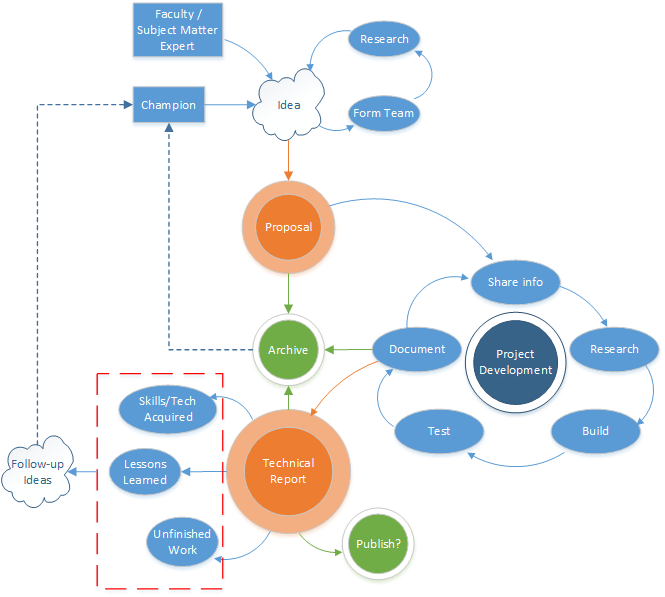
\includegraphics[width=\linewidth]{figs/project-life-cycle.png}
%  \caption{A PDD is the first piece of documentation to be archived in the project life cycle. Since the life cycle can be iterative, a new design document may also refer to one or more previous SPPs.}
%\label{fig:lifecycle}
%\end{figure}

% \section{Secondary Objectives}
% \label{sec:secondary-obj}
% Secondary Objectives are lower priority or bonus objectives that are significant but not the main focus of the project. This template does not have secondary objectives.


\section{Benefit to SPEX}
\label{sec:benefit}
% One of the core values of SPEX is to provide opportunities for academic and professional growth for its members,
% and to challenge them with interesting projects.
% In this section, explain how the project would benefit SPEX members as students,
% space enthusiasts, and young professionals.

The benefits to SPEX are two-fold.  Firstly this will give the members new tools and technologies to conduct astro tracking related research.  Secondly it will provide items for the astro tracking team to showcase at events like Imagine RIT.

\subsection{New Technologies and Equipment}
    \subsubsection{Tracking Mount}
    \label{sec:trackingmount}
    Mount to assist in astrophotography without telescope will allow for students to take pictures that were otherwise not able to be taken with current equipment.
    \subsubsection{Orion Mount}
    \label{sec:orionmounts}
    Extra telescope mount to use during star-gazing sessions will allow more students to get hands on experience with the telescopes when they are taken out.
    \subsubsection{Tracking Software}
    \label{sec:trackingmounts}
    Software to help with tracking of artificial satellites will allow members to conduct research in the future.

\subsection{Showcase Pieces for Imagine}
\label{sec:showcasepieces}
Two new mounts will be developed which are physical items that can be used to start conversation with event attendees.  This will appeal to more mechanical individuals who are not directly interested in software.
New pictures will also be taken that will outline the capabilities of both the members and the new technologies developed. These showcase pieces will help improve the credibility of the RIT SPEX Astro Tracking team and increase the chances of future sponsorship for SPEX as a whole.


\section{Implementation}
\label{sec:implementation}
  % What path do you anticipate the project to take?



\subsection{Timeline}
\label{subsec:timeline}
    \subsubsection*{Week 3}
    Project plans.  An outline of the steps each team will take to complete their sub-project
    \subsubsection*{Week 5-7}
    Progress Updates. Update on progress of project
    \subsubsection*{Week 8}
    Mid presentation.  Give an in-depth analysis of the project.  Will outline project status, roadblocks, and what is left to do.
    \subsubsection*{Week 12}
    Projects ideally will be completed, or near-completion, at this point for showcasing at Imagine RIT.



\subsection{Deliverables}
\label{subsec:deliverables}

Deliverable items for this project include a small mid-semester presentation to outline where each of the projects are at and what needs to be done in order to complete them.  Then each team will deliver their final projects.  For each of the mount teams their respected mounts will be the delivery.  The tracking mount should also present pictures taken of celestial objects to indicate it works as desired.  The team working on the software will provide the finished code as well as a presentation outlining how to use it, how it works, as well as the technologies used.  Lastly the research team will present their findings to the group as well as create a small paper that will be reviewed by the team and, ideally, be pushed forth for publication.




\section{Externalities}
  % Things not directly related to the work or outcomes, but related to the project as a whole.
\subsection{Prerequisite Skills}
  % Which skills do team members need to have before work can start (not including skills that will be learned ``on the job'')?
Many of these projects are interdisciplinary but between them will require from ten to twelve members.  Each respected team will get anywhere between two to four members depending on the complexity and skill set of each team.  Ideally for the mounts there should be an upperclassman mechanical engineer.  For the research team there should be at least one physics related major.  Lastly for the software team it will be recommended to have one member familiar with orbital mechanics and another with general software development.


\subsection{Funding Requirements}
  % Estimate costs that would be needed to meet objectives.
Funding requirements for these projects should be kept to a minimum.
The mount teams will not exceed 50 dollars in materials for each respective mount and the software/research teams will require no additional funding.


\subsection{Faculty Support}
  % Identify faculty that will be involved (or would need to be involved) to meet objectives.
  % Note that if a professor is the Principal Investigator (P.I.) for a project, there still needs to be a student as the SPEX Project Champion.
No faculty have explicitly expressed interest in these projects. However they can be consulted if questions do arise in any stage of development.  While it is certainly feasible to do these projects without professor help it would greatly benefit the members to develop relationships with professors to help in development.

\subsection{Long-Term Vision}
\label{sec:vision}
Once new technologies are developed the Astro Tracking team will be better prepared to conduct research in the future.  The mounts allow for obtaining better data during observations, the software will allow for the pursuit of tracking artificial satellites, and the research team will help provide a framework for how to conduct future research.

\section*{Acknowledgements}
The Author would like to thank all sponsors, current members who dedicate their hard work and time, and all faculty advisors for RIT SPEX.


\bibliographystyle{IEEEtran}
\bibliography{sample-with-examples}

%\onecolumn
%\appendices{}
%\section{Project Life Cycle}
%\begin{figure}[h]
%  \centering
%  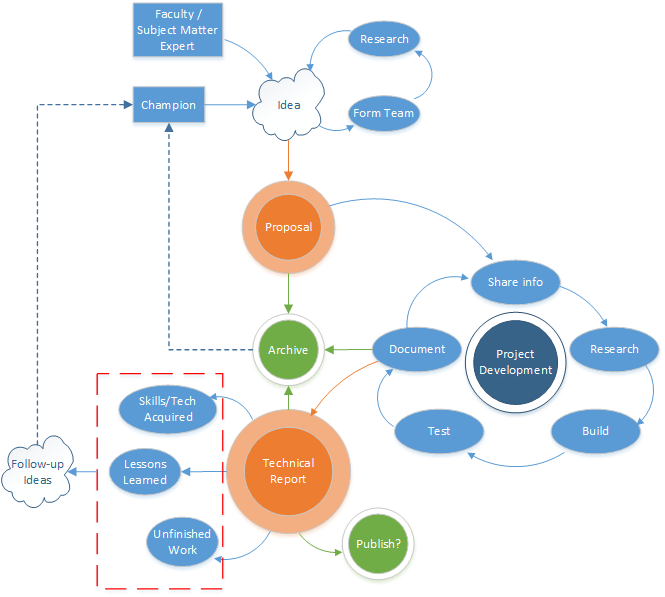
\includegraphics[]{figs/project-life-cycle.png}
%  \caption{Enlarged version of the diagram in \autoref{fig:lifecycle}.}
%\end{figure}

\end{document}
